\question
(0,5 балла) В офисе ООО “Рога и копыта” стоит удивительная сеть маршрутизаторов, коммутаторов и прочего связного барахла. В серверной не прибирались с момента основания, и вам выпала честь навести порядок. Вы решаете начать с проводов, надо бы разложить их красиво. На данный момент ситуация следующая:

\begin{minipage}[h]{0.45\linewidth}
\center{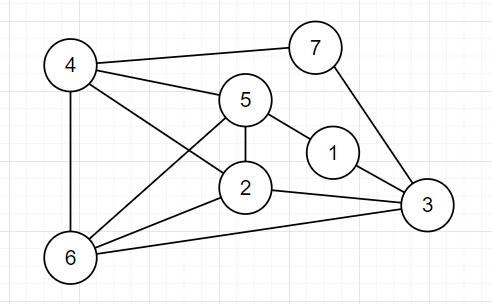
\includegraphics[width=0.7\textwidth]{pic/96.png} }
\end{minipage}

где вершина — какой-либо прибор, ребро — провод между приборами.

Можно ли уложить провода так, чтобы провода не пересекались?
